\documentclass[12pt,a4paper,openany]{book}
\usepackage[utf8]{inputenc}
\usepackage[T1]{fontenc}
\usepackage{amsmath,esint}
\usepackage{amsfonts}
\usepackage{mathrsfs}
\usepackage[british,UKenglish,USenglish,english,american]{babel}
\usepackage[Glenn]{fncychap}
\usepackage{amssymb}
\usepackage[left=1cm,right=1cm,top=1.5cm,bottom=1.5cm]{geometry}
\usepackage{fancyhdr}
\pagestyle{fancy}
\usepackage{pifont}
\usepackage{array}
\usepackage{multirow}
\usepackage[dvipsnames]{xcolor}
\usepackage{hyperref}
\renewcommand{\thesection}{\Roman{section})}
\renewcommand{\thesubsection}{\arabic{subsection})}
\renewcommand{\thesubsubsection}{\alph{subsubsection})}
\usepackage{xeboiboites}
\usepackage{graphicx}
\usepackage[version=4]{mhchem}
\usepackage{tcolorbox}
\def\nbR{\ensuremath{\mathrm{I\! R}}}
\def\nbN{\ensuremath{\mathrm{I\! N}}}
\def\nbK{\ensuremath{\mathrm{I\! K}}}

\usepackage{listings}
\usepackage{color} %red, green, blue, yellow, cyan, magenta, black, white

\definecolor{darkWhite}{rgb}{0.94,0.94,0.94}

\definecolor{lightgray}{rgb}{.9,.9,.9}
\definecolor{darkgray}{rgb}{.4,.4,.4}
\definecolor{purple}{rgb}{0.65, 0.12, 0.82}

\lstdefinelanguage{JavaScript}{
  keywords={typeof, new, true, false, catch, function, return, null, catch, switch, var, if, in, while, do, else, case, break},
  keywordstyle=\color{blue}\bfseries,
  ndkeywords={class, export, boolean, throw, implements, import, this},
  ndkeywordstyle=\color{darkgray}\bfseries,
  identifierstyle=\color{black},
  sensitive=false,
  comment=[l]{//},
  morecomment=[s]{/*}{*/},
  commentstyle=\color{OliveGreen}\ttfamily,
  stringstyle=\color{OliveGreen}\ttfamily,
  morestring=[b]',
  morestring=[b]"
}

\lstset{
  aboveskip=3mm,
  belowskip=-2mm,
  xleftmargin=15pt,
  backgroundcolor=\color{darkWhite},
  basicstyle=\footnotesize,
  breakatwhitespace=false,
  breaklines=true,
  captionpos=b,
  commentstyle=\color{OliveGreen},
  deletekeywords={...},
  escapeinside={\%*}{*)},
  extendedchars=true,
  framexleftmargin=0pt,
  framextopmargin=3pt,
  framexbottommargin=2pt,
  frame=tb,
  keepspaces=true,
  keywordstyle=\color{blue},
  language=C++,
  literate=
  {²}{{\textsuperscript{2}}}1
  {⁴}{{\textsuperscript{4}}}1
  {⁶}{{\textsuperscript{6}}}1
  {⁸}{{\textsuperscript{8}}}1
  {€}{{\euro{}}}1
  {é}{{\'e}}1
  {è}{{\`{e}}}1
  {ê}{{\^{e}}}1
  {ë}{{\¨{e}}}1
  {É}{{\'{E}}}1
  {Ê}{{\^{E}}}1
  {û}{{\^{u}}}1
  {ù}{{\`{u}}}1
  {â}{{\^{a}}}1
  {à}{{\`{a}}}1
  {á}{{\'{a}}}1
  {ã}{{\~{a}}}1
  {Á}{{\'{A}}}1
  {Â}{{\^{A}}}1
  {Ã}{{\~{A}}}1
  {ç}{{\c{c}}}1
  {Ç}{{\c{C}}}1
  {õ}{{\~{o}}}1
  {ó}{{\'{o}}}1
  {ô}{{\^{o}}}1
  {Õ}{{\~{O}}}1
  {Ó}{{\'{O}}}1
  {Ô}{{\^{O}}}1
  {î}{{\^{i}}}1
  {Î}{{\^{I}}}1
  {í}{{\'{i}}}1
  {Í}{{\~{Í}}}1,
  morekeywords={*,...},
  numbers=left,
  numbersep=6pt,
  numberstyle=\tiny\color{black},
  rulecolor=\color{black},
  showspaces=false,
  showstringspaces=false,
  showtabs=false,
  stepnumber=1,
  stringstyle=\color{OliveGreen},
  tabsize=4,
}



%% Table des matières
\setcounter{secnumdepth}{3}
\setcounter{tocdepth}{3}



%%maccros
\newcommand{\rot}{\overrightarrow{\mathrm{rot}}}
\renewcommand{\div}{\mathrm{div}}
\newcommand{\grad}{\overrightarrow{\mathrm{grad}}}
\newcommand{\dt}{\mathrm{d}t}
\newcommand{\dd}{\mathrm{d}}
\newcommand{\esp}{\noalign{\vspace{4pt}}}
\newcommand\scr[1]{\mathscr{#1}}
\newcommand\para{\,/\!/\,}
\newcommand\C{(\scr{C})}
\newcommand\e{\mathrm{e}}
\newcommand\m{\vec{\scr{M}}}
\newcommand\scre{\scr{S}_{cr\acute e\acute ee}}
\newcommand\sech{\scr{S}_{\acute ech}}
\newcommand\dv{{D_V}_{(S)}}
\newcommand\dm{{D_m}_{(S)}}


% Header
\lhead{Chambelin Kévin}
\chead{Real Time Systems}
\rhead{Bus Project}


% Boite définition :
\newbreakabletheorem[small box style={fill=blue!20,draw=black, rounded corners},big box style={fill=blue!10,draw=black,thick,rounded corners},size={\linewidth},headfont={\bfseries},thcounter=chapter]{definition}{Définition}{defcounter}
\renewcommand{\thedefcounter}{\arabic{defcounter}}

% Boite théorème :
\newbreakabletheorem[small box style={fill=red!20,draw=black, rounded corners},big box style={fill=red!10,draw=black,thick,rounded corners},size={\linewidth},headfont={\bfseries},thcounter=chapter]{function}{Function}{thmcounter}
\renewcommand{\thethmcounter}{\arabic{thmcounter}}
% Boite proposition :
\newbreakabletheorem[small box style={fill=green!20,draw=black, rounded corners},big box style={fill=green!10,draw=black,thick,rounded corners},size={\linewidth},headfont={\bfseries},thcounter=chapter]{proposition}{Proposition}{propcounter}
\renewcommand{\thepropcounter}{\arabic{propcounter}}
% Boite remarques :
\newbreakabletheorem[small box style={fill=white!10,draw=none, rounded corners},big box style={fill=white!10,draw=none,thick,rounded corners},size={\linewidth},headfont={\bfseries},thcounter=chapter]{remarque}{\ding{43} Observation}{remcounter}
\renewcommand{\theremcounter}{\arabic{remcounter}}

% Boite exemple :
\newbreakabletheorem[small box style={fill=white!20,draw=white, rounded corners},big box style={fill=white!10,draw=white,thick,rounded corners},size={\linewidth},headfont={\bfseries},thcounter=chapter]{exemple}{\ding{46} Exemple}{excounter}
\renewcommand{\theexcounter}{\arabic{excounter}}

% Boite propriété :
\newbreakabletheorem[small box style={fill=green!20,draw=black, rounded corners},big box style={fill=green!10,draw=black,thick,rounded corners},size={\linewidth},headfont={\bfseries},thcounter=chapter]{strategy}{Strategy}{proprcounter}
\renewcommand{\theproprcounter}{\arabic{proprcounter}}

% Boite démonstration :
\newbreakabletheorem[small box style={fill=white!20,draw=black, rounded corners},big box style={fill=white!10,draw=black,thick,rounded corners},size={\linewidth},headfont={\bfseries},thcounter=chapter]{demo}{Démonstration}{}

% Boite answer :
\newbreakabletheorem[small box style={fill=gray!20,draw=black, rounded corners},big box style={fill=gray!10,draw=black,thick,rounded corners},size={\linewidth},headfont={\bfseries},thcounter=chapter]{answer}{Answer}{}



\begin{document}
%% Titre
\begin{tcolorbox}[arc=1ex, left=3pt, right=3pt, top=3pt, bottom=2pt]
  \center \LARGE \textbf{Real Time Systems -- Bus project}
\end{tcolorbox}
\bigskip
\section*{Introduction}
\hspace*{0.6cm}My project was to implement a website to manage a bus company, with the possibility for clients to reserve bus seats.\\

The main difficulty of this project is the number of languages it requires : PhP, SQL, JavaScript (js), Html, CSS, and finally, Cpp.\\

To implement this website, I used the Laravel framework. It allows greater possibilities than coding all the website from scratch. It facilitates the communication between html, php, js, css and sql.\\

Up to this point, the actual difficulty is to handle real time system with Cpp. In fact, it could have been achieved by Php, that has tools similar to Cpp mutex. But, for this project, the aim was to implement it in Cpp. And it is at this moment that comes the higher difficulty of this project: made the website and the Cpp code communicate with each other. I will explain how I managed to do that later in this report.

\begin{remarque}
	The pictures can be a bit small. You can find the original ones in the following folder :\\
	\emph{bus\_project/Report/Figs}\\
	They are named \emph{fig\{x\}}, in the order of the report.
\end{remarque}

\begin{remarque}
	This website needs a server to run, the Cpp part and the database part too. I can't let them run all the time because I have an other website I'm working on runnning on my serser, and it does not like when both are launched... If you want to visit the website by yourself on your browser, please feel free to send me an email, and I will turn it on a few hours. I hope you'll understand.
\end{remarque}

\begin{remarque}
	I've tried to put the code into the report, but sometimes, it is not very easy to read. It might be easier for you to open the good file in parallel.
\end{remarque}

\begin{remarque}[Important -- Link to the github repository]
You can find all the files here: \color{blue}\href{https://github.com/kchambelin/Bus}{click here}\color{black}\\

It should be public so that you can read and download files. If you don't, feel free to email me.
\end{remarque}

\tableofcontents
\newpage

\section{The global architecture of the website}
\subsection{A website...}
The website is composed of two public pages : the home page, and the bus page. The home page is not very useful. It is just to present the company. However the bus page is the main page of the website: it allows the user to see the current buses and to reserve seats.

\begin{center}
	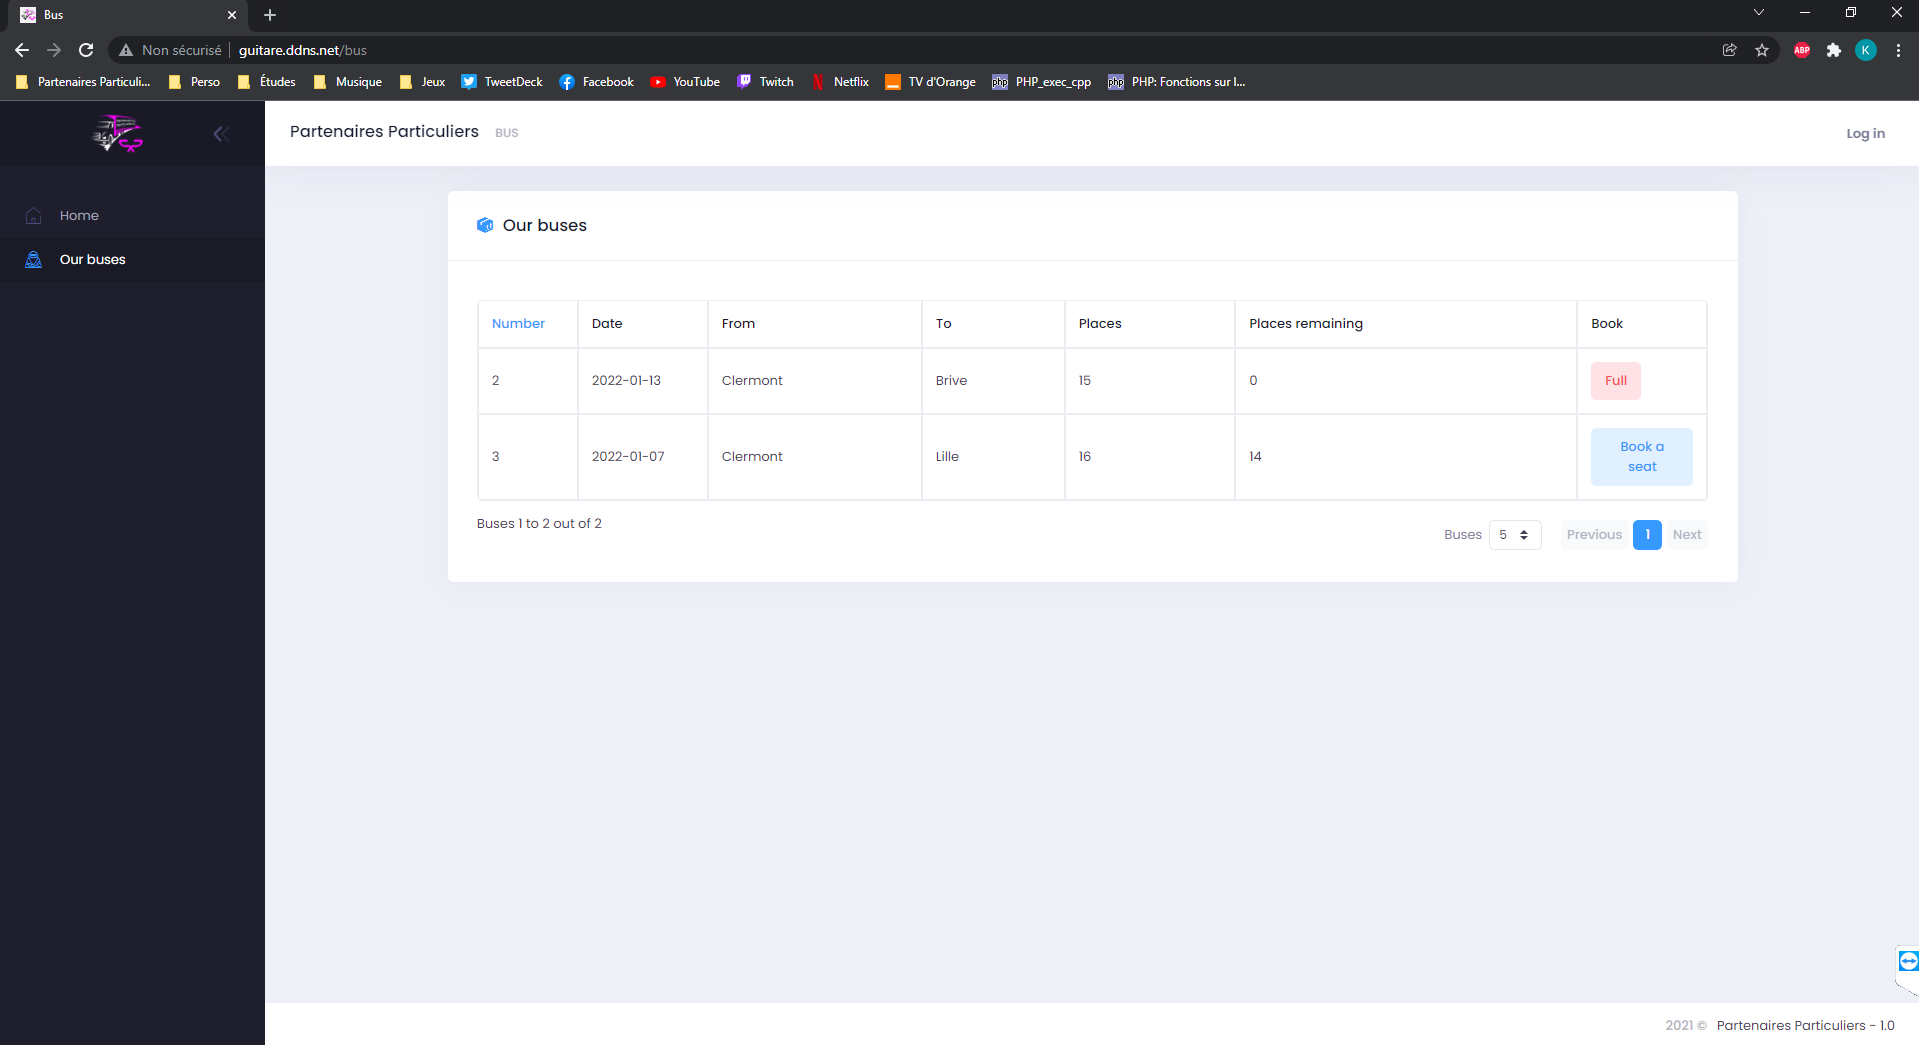
\includegraphics[scale=0.35]{Figs/fig1}
\end{center}

There is also a other page called \emph{Manage bus}, that is for the owner of the company (that I will call Admin). This page allows the admin to create a bus.

\begin{center}
	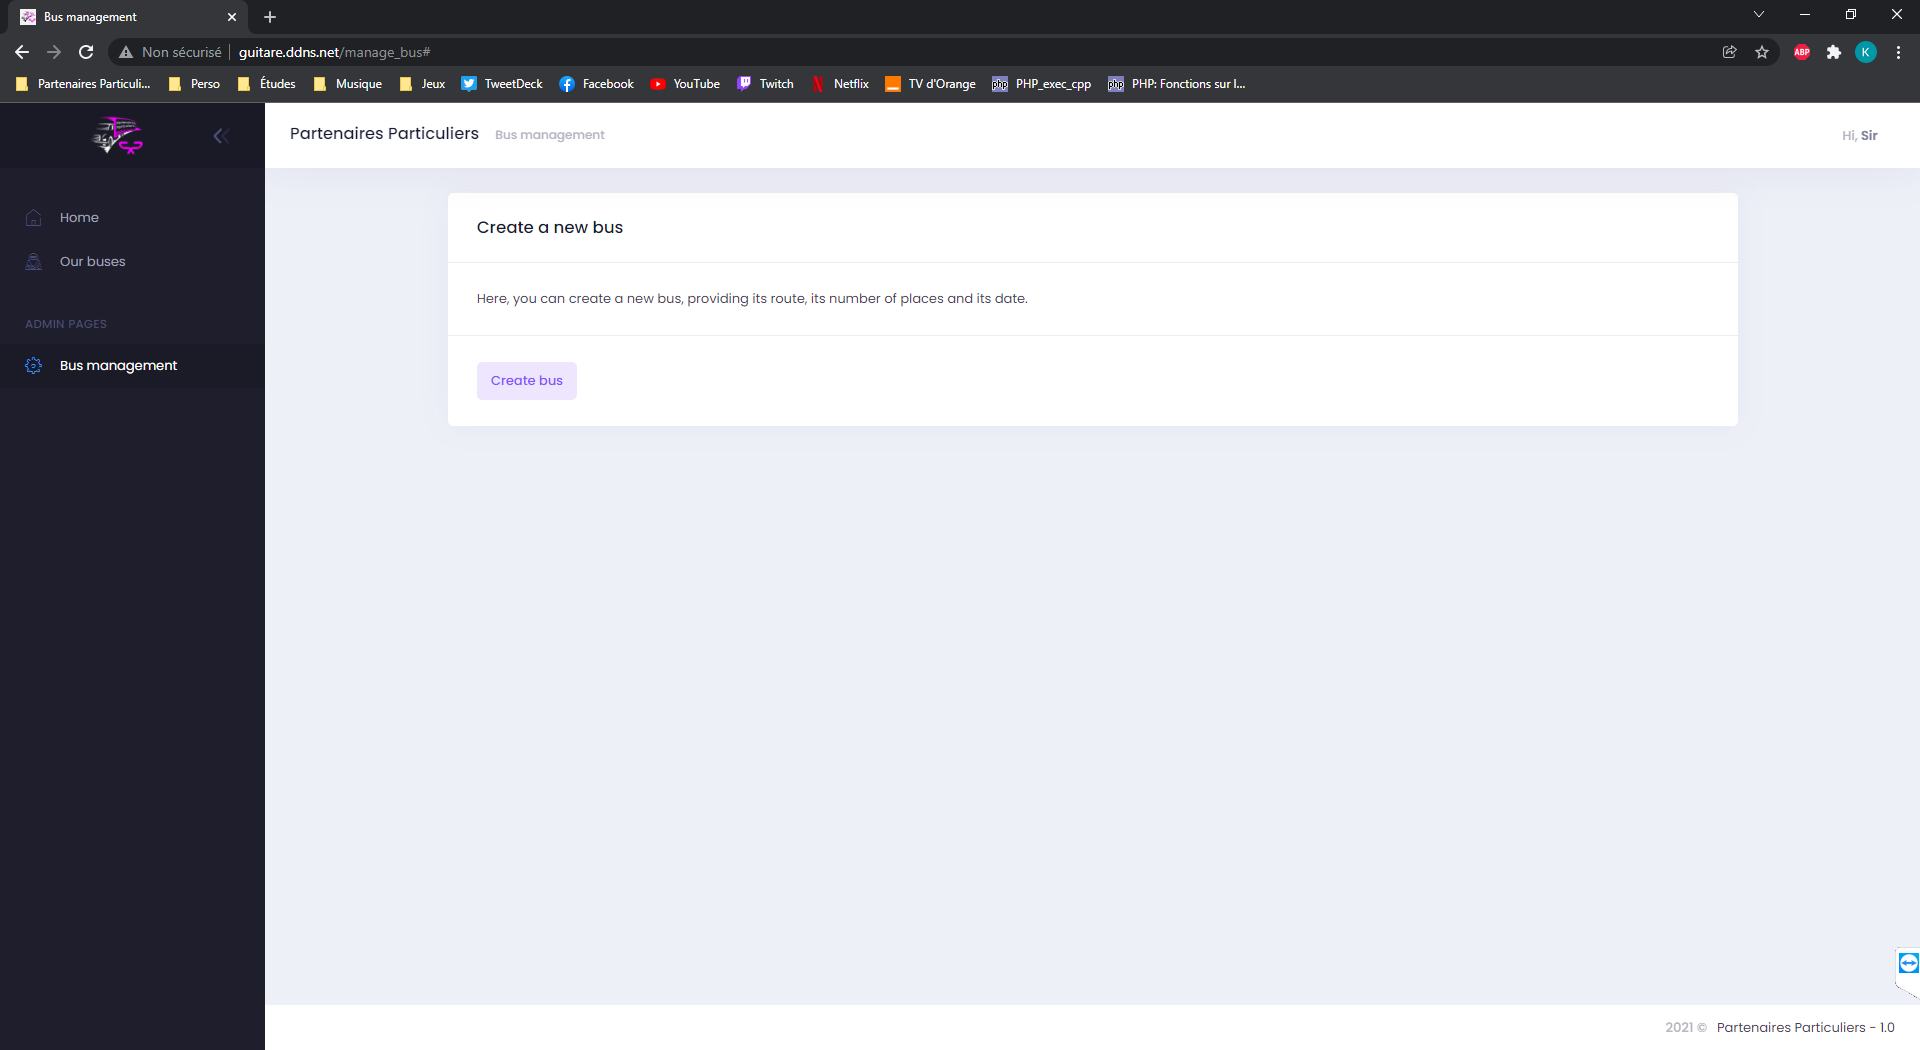
\includegraphics[scale=0.35]{Figs/fig2}
\end{center}

As you may have noticed, there is a difference in the navigation list between the both images: the manage bus page is not visible if your are not an admin. It is handled by a system of permissions.
\pagebreak

But to know if you are an admin or not, you need to have an account. So, there is a page dedicated to login and registration, accessible by the Log in button, on the right.

\begin{center}
	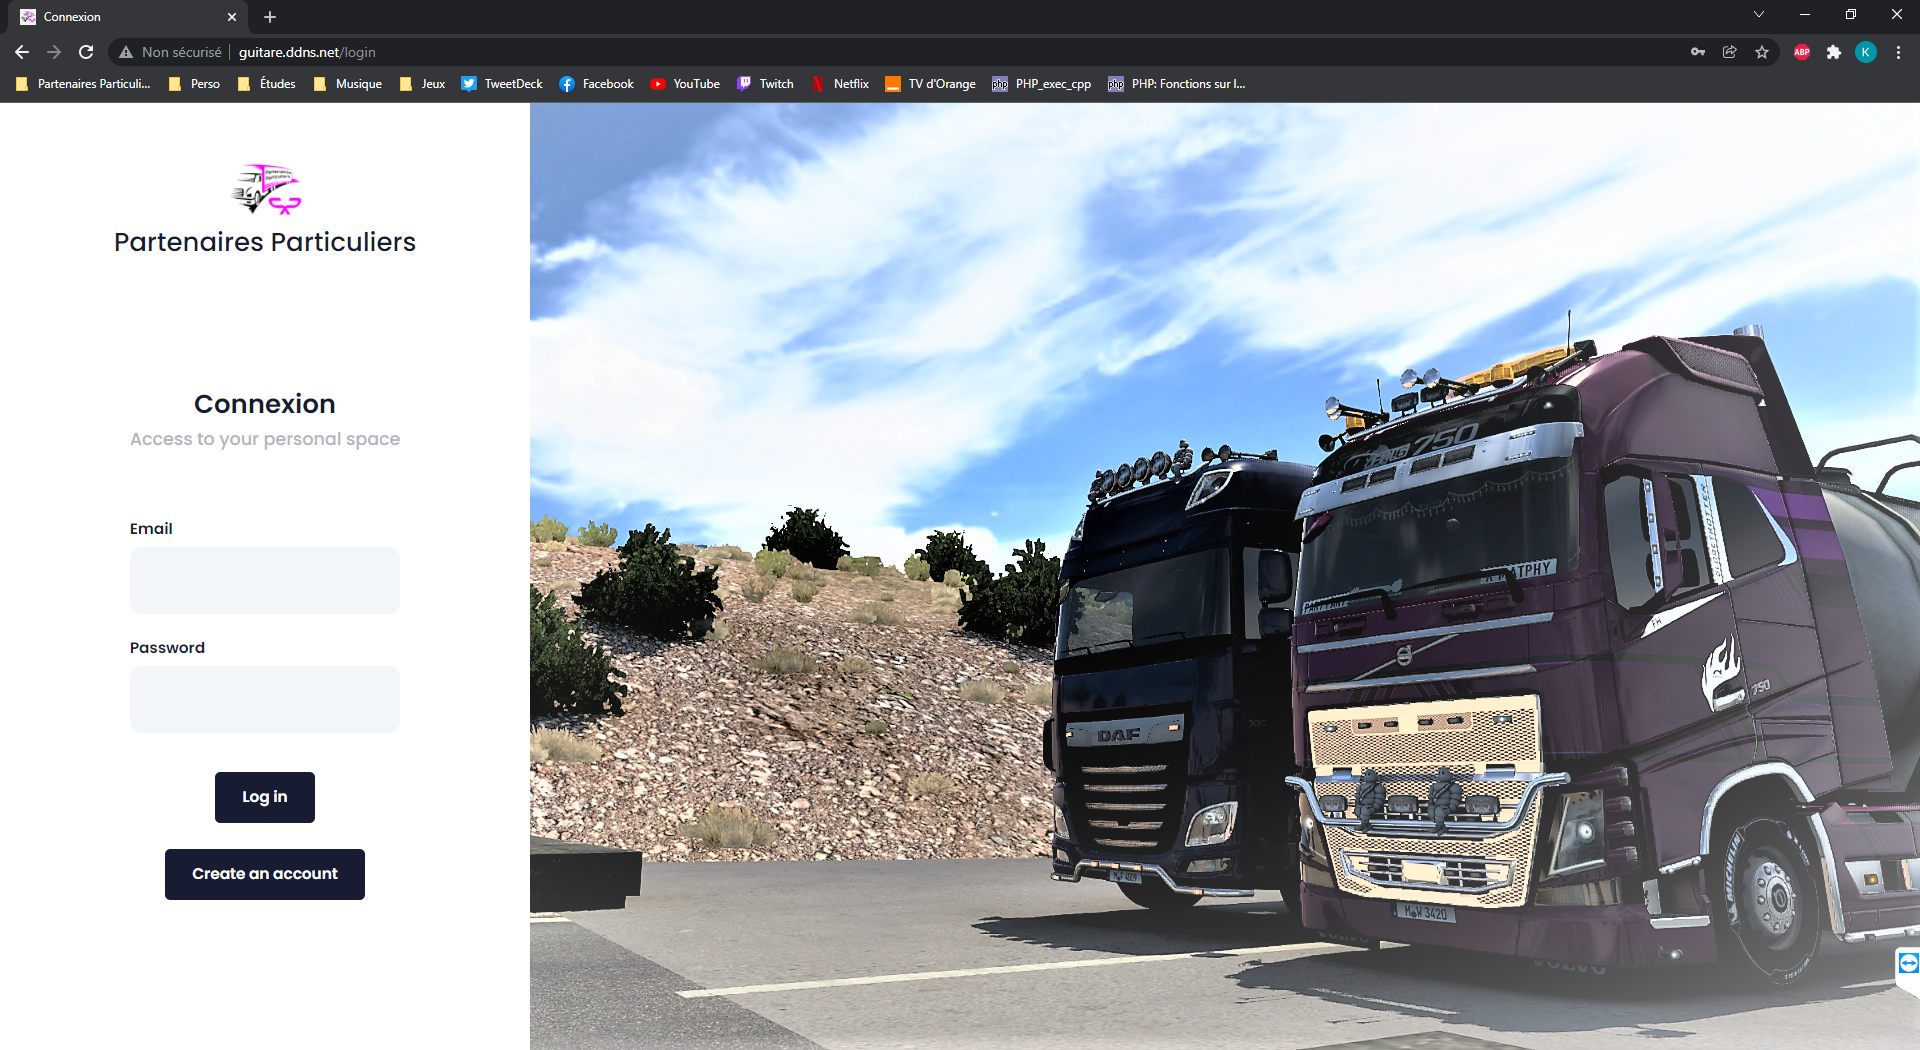
\includegraphics[scale=0.35]{Figs/fig3}
\end{center}

In case you don't have any account yet, you can register here :

\begin{center}
	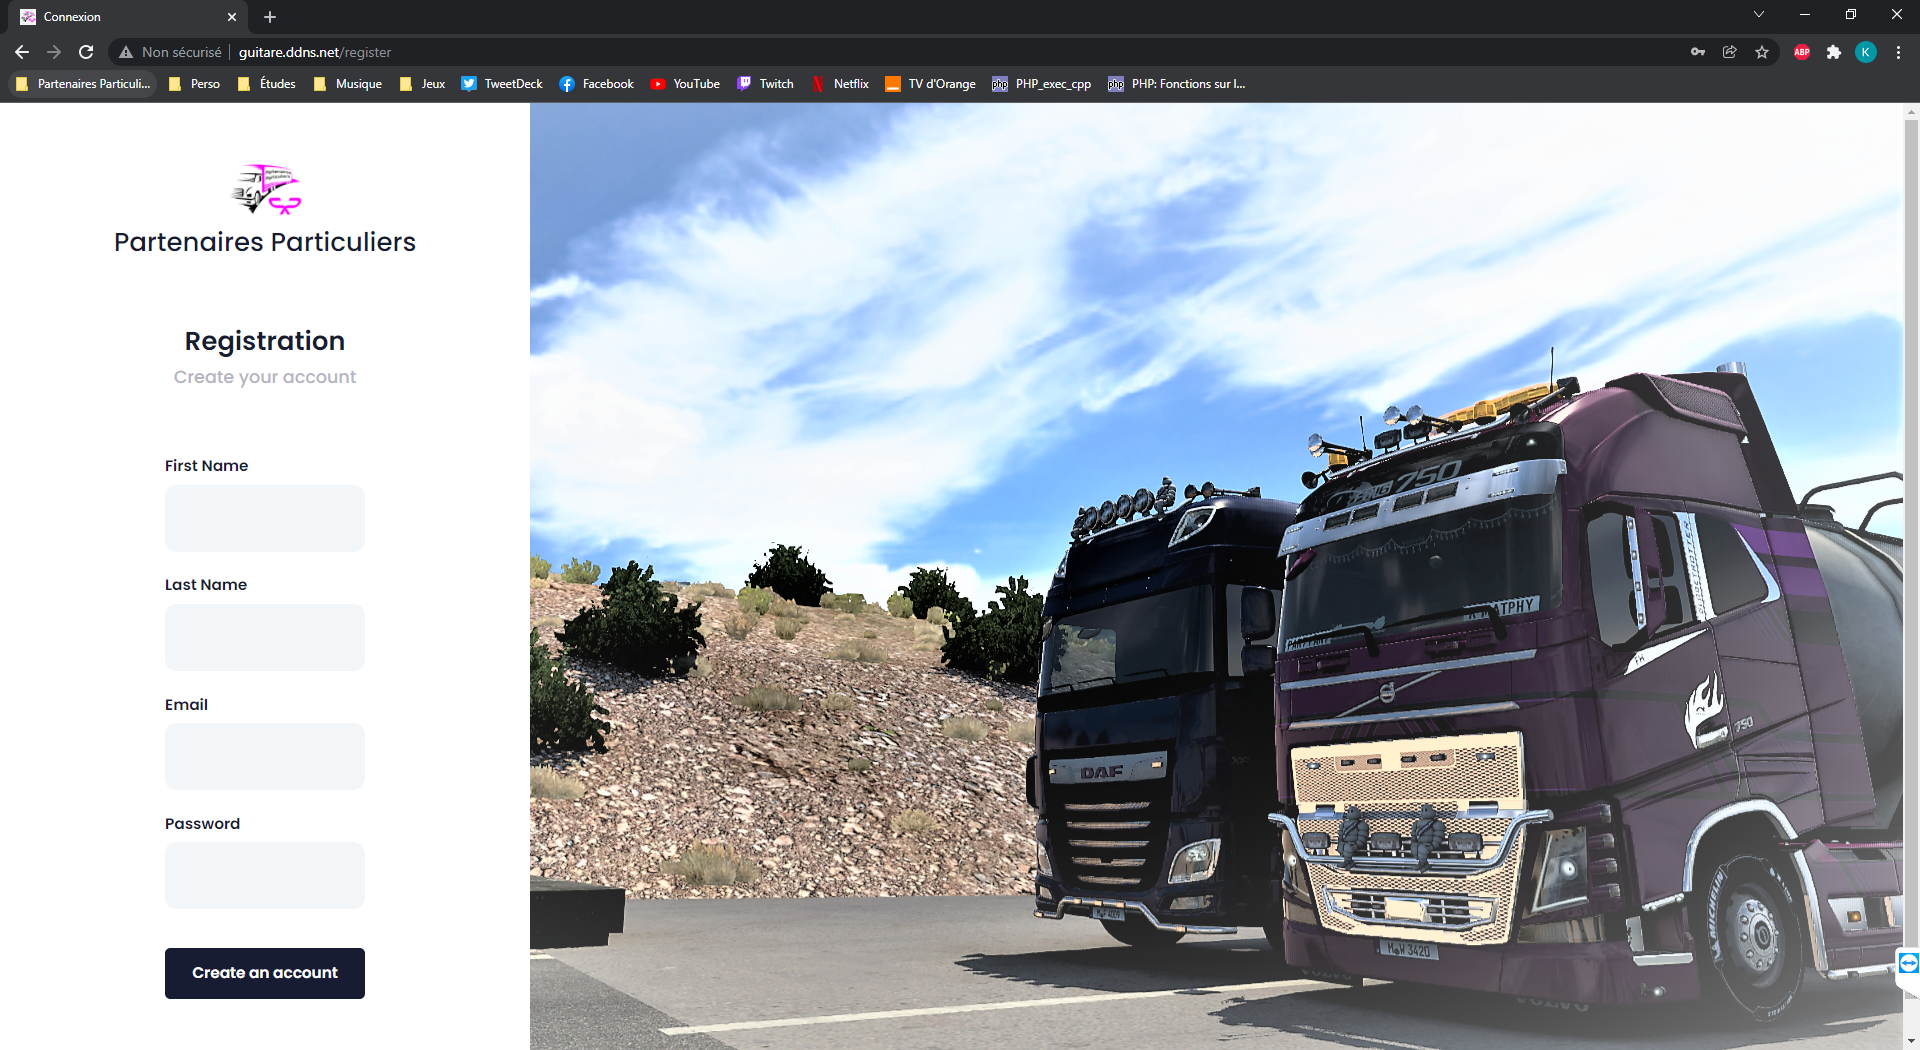
\includegraphics[scale=0.35]{Figs/fig4}
\end{center}

\begin{remarque}
	You may ask yourself why there are trucks here, instead of buses. The fact is that I already have a working website about a virtual trucks company. I've been working on this website for one year now, so I reuse some pieces of  my code to save some time for this project. It why there are Trucks, or why the name is a French one.
\end{remarque}

\subsection{...but not alone}
To make this website work well, it requires some other things. Indeed, we talked about accounts, permissions, buses... All of these have to be stored somewhere. It is why we need a database. This database will store all the data required by the website.\\
The other important thing to have is the Cpp server, that will handle the synchronisation part.

\section{The database}
The database is a MySQL database.
\subsection{Create the database}
I have worked a lot with database (db), and although there are some softwares than provide way to work on db without any SQL commands, I think that is more efficient and rigorous to use only commands. So to create the database, I used a script that you can find here:\\
\emph{bus\_project/DB/Creation\_Script.sql}\\

The first part of the script is the following:
\lstinputlisting[language=SQL, firstline=1, lastline=6, firstnumber=1]{../DB/Creation_Script.sql}
\bigskip
In fact, it is the last part that we write when you are doing this script, because it is a kind of protection part in case of failure when you execute the script. What is it doing? The word \emph{drop} means delete, so the first line will delete the table bus. But there is \emph{if exists}. So, it checks if the table bus exists. If yes, it drops it, if no, it does nothing. This part ensures you that you are not messing up your tables and that there are clean.\\

The next part is the creation of the tables:
\lstinputlisting[language=SQL, firstline=9, lastline=54, firstnumber=9]{../DB/Creation_Script.sql}
\bigskip
SQL is quite transparent. \emph{CREATE TABLE} means that we create the table bus. Then, between the parenthesis, we define all the attributes of the table. I will explain for the bus table:
\begin{itemize}
	\item idbus, which is an integer and cannot be null.
	\item date, which is saved as a date format and cannot be null.
	\item from\_city, which is a varchar(50), that is a string that can be 0-50 long and cannot be null.
	\item to\_city, which is a varchar(50), that is a string that can be 0-50 long and cannot be null.
	\item place\_number, which is an integer and cannot be null.
\end{itemize}
Up to this point, we have our tables. But if we want them to work efficiently, we need to declare two things:
\begin{itemize}
	\item the primary key of each table: the attribute that is unique for each row, and allows to identify the data.
	\item the foreign key if necessary: it is when a table refers to the primary key of another table, like for exemple, in the table books, bus\_idbus that refers to idbus of the table bus. Foreign keys are very helpful to do joins between tables.
\end{itemize}
We do that this way:
\lstinputlisting[language=SQL, firstline=56, lastline=73, firstnumber=56]{../DB/Creation_Script.sql}
\bigskip
In this script, the declarations are done table by table. The first line declares the primary key, and then, if necessary, the foreign keys.

\subsection{Tables glossary}
\subsubsection{Table users}
In this table, we will have the registration data for each user:
\begin{itemize}
	\item iduser, the id of the user,
	\item email, the email of the user,
	\item grade, the level of rights (0: normal user, 1: admin),
	\item password, the password of the user.
\end{itemize}
\begin{remarque}
	For security purpose, the password is encoded before being stored. For exemple, if the password is "real-time systems", in the db, we will have a hash version of the password.
\end{remarque}

\subsubsection{Table user\_details}
In this table, we will have the personal data of each user.
\begin{itemize}
	\item iduser\_detail, the primary key.
	\item users\_iduser, the foreign key that refers to the primary key of the table users.
	\item firstname, the firstname of the user.
	\item lastname, the lastname of the user.
\end{itemize}
\begin{remarque}
	I could have put this data into the users table, because it's a little website with not so much data. But I learned from my other project that is better to keep the registration data together and to add another table with personal data.
\end{remarque}

\subsubsection{Table operations}
This table is used to define the actions people can do on the website. We have:
\begin{itemize}
	\item idoperation, the primary key.
	\item name, name of the operation.
	\item description, description of the operation (not mandatory but useful with huge projects).
	\item route, the route that is concerned by the operation (can be null). I'll explain what a route is later.
\end{itemize}

\subsubsection{Table permissions}
This table says which grade can do which operation. We have:
\begin{itemize}
	\item idpermission, the primary key.
	\item grade, the concerned grade.
	\item operations\_idoperation, the foreign key refering to operations.
\end{itemize}

\subsubsection{Table tokens}
When you are logged into the website, you have a unique token. It is stored here:
\begin{itemize}
	\item idtoken, the primary key.
	\item users\_iduser, the foreign key that refers to users.
	\item token, the token itself.
\end{itemize}

\subsubsection{Table bus}
The table that has all the data of a bus:
\begin{itemize}
	\item idbus, the primary key.
	\item date, the date of the bus.
	\item from\_city, the city the bus comes from.
	\item to\_city, the city the bus will go.
	\item place\_number, the number of places in the bus.
\end{itemize}

\subsubsection{Table books}
This table will contains all the seats bought by the users. Each time the user by a seat, it will add a new line. We have:
\begin{itemize}
	\item idbook, the primary key.
	\item bus\_idbus, the foreign key that refers to bus.
	\item users\_iduser, the foreign key that refers to users.
\end{itemize}

\section{The website part}
\subsection{Global architecture using Laravel Framework}
\begin{minipage}{0.2\linewidth}
\begin{center}
	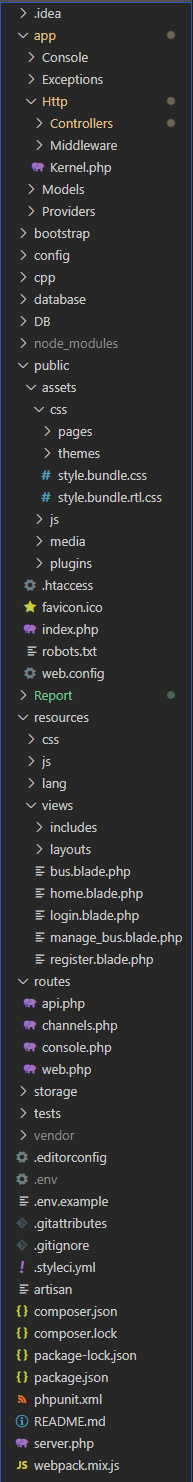
\includegraphics[scale=0.65]{Figs/fig5}
\end{center}
\end{minipage}\hfill
\begin{minipage}{0.8\linewidth}
	As you can see, there are many folders and files to make all of this work.\\
	
	There are some important aspects about developing this kind of application:
	\begin{itemize}
		\item the pages themselves: there are stored in \emph{bus\_project/resources/views}. They are .blade.php files.
		\item the routes: it's like an itinerary for each data, each command, each function. The ones I've done are in two files : \emph{bus\_project/routes/api.php} and \emph{bus\_project/routes/web.php}
		\item the CSS file: it contains all the parameters about the graphic interface. \emph{bus\_project/public/assets/css/style.bundle.css}
		\item the controllers: there are php files where are the main functions I've implemented about my application. The idea is to call them from the page file using AJAX. I'll talk about it later. \emph{bus\_project/app/Http/Controllers}
		\item the middleware: there are like controllers but more deeper in the application. While controllers do things like reserve a seat, the middleware will take care about connections, permissions, stuffs like this. \emph{bus\_project/app/Http/Middleware}
		\item the models: there are files which represent the tables of the db. There are used to help the website communicate with the db. \emph{bus\_project/app/Models}
	\end{itemize}
	\begin{remarque}
		You can find some scripts about the db in \emph{bus\_project/DB}.\\
		You can find the cpp file in \emph{bus\_project/cpp}.
	\end{remarque}
\end{minipage}

\subsection{The login system}
\subsubsection{The login page}
To understand the login part, the important part of the login.blade.php is the following:
\lstinputlisting[language=html, firstline=57, lastline=117, firstnumber=57]{../resources/views/login.blade.php}
\bigskip
The first part (l.60 - l.79) is checking if the user has already been logged. If yes, it redirects to the home page, with as a logged user. Otherwise, it displays the error (for example, wrong password).\\
Then, we can find the form group, that is the part where we enter our email and password. Then, we can submit it (l. 108).\\
If we do not have account now, we can use the button Create an account (l. 111).

\begin{remarque}
	About the link to the creation of account, we can say that we call the route register, instant of calling directly a page.
\end{remarque}

\subsubsection{Login management}
The main part of the login system is directly handled by Laravel. So, I won't talk about it. We just have to know that we can access to the connected user by \emph{Auth::user()}.

\subsubsection{Creating an account}
This process was completly done by hand, so I will explain it. Once you arrive to the register page, you can see a form. In Php/Html, we have:
\lstinputlisting[language=html, firstline=62, lastline=98, firstnumber=62]{../resources/views/register.blade.php}
\bigskip
As you can see, every form is implemented as an html <input>. Each of them has an id. It's important for them to have a different id.\\

At the end, we have the Create an account button. What is important with it is the \emph{onclick = "Create\_user()"}. It means that when you click on the button, it will call the js function declared in the script part at the end of the file, which is:
\lstinputlisting[language=javascript, firstline=128, lastline=154, firstnumber=128]{../resources/views/register.blade.php}
\bigskip

Here we are! The first AJAX function. What is it exactly? It's a way to send data from the client side (the js function) to the server side (the php controller).\\


The first line add a spinner to the button, so that the user sees something is happening.\\*

Then, we define the AJAX itself:
\begin{itemize}
	\item the url is the route to the controller function.
	\item the type is what we are doing: POST => send to the server, GET => receive from the server.
	\item headers: the token. Here it's a little bit tricky because the user does not have a token yet.
	\item data: all the attributes we want to pass to the php function.
	\item the success function: what does the js function after the ajax function responded ? Here it redirects to the login page.
\end{itemize}
\begin{remarque}[Warning!]
	An AJAX function is an asynchronous function!
\end{remarque}
\begin{remarque}
	The js (aka the client) does not have any access to the database. It's only the php (aka the server). So, we need to transfer the data to the php.
\end{remarque}
\begin{remarque}
Let's see the code of the route, in the web.php file:
\lstinputlisting[language=php, firstline=51, lastline=51, firstnumber=51]{../routes/web.php}
\bigskip
How is it built? It's a route so Route::. Then, it's a post type, so post. Then the name of the route ('user/create'), then the address of the controller. Finally, after the @, it is the name of the function inside the controller file.
\end{remarque}
Let's see the controller function now, in \emph{bus\_project/app/Http/Controllers/Auth/CreateUserController.php}:
\lstinputlisting[language=php, firstline=3, lastline=95, firstnumber=3]{../app/Http/Controllers/Auth/CreateUserController.php}
\bigskip
The first part, from line 3 to 11, is the equivalent of the \#include in Cpp.\\

Then in the controller part, we have two functions, the function Create, that is called by the AJAX function, and the function gen\_uuid, that will be called by the create function.\\

So, about the Create function:

The first part of the function is to get the data sent by the AJAX function. There are in the Request object. So we need the 18 to 21 lines to store them into php variables.

\begin{remarque}
	In PHP, there is a \$ before a variable name.
\end{remarque}
Then, we assess that the password is alphanumerical, because Laravel just knows how to handle alphanumerical ones.\\

The next part is to get from the table users the last id.

\begin{remarque}[About SQL with Laravel]
	Usually, to get the last id, we would have execute:
	
	\emph{SELECT MAX(iduser) FROM users}.\\
	But Laravel provides a Query Builder, that is more secure. The difficulty is that instead of executing a request, it is more like a table was an object. So, the request becomes:
	
	\emph{Users::orderBy('iduser','desc')->first->iduser}\\
	The SQL equivalent is :
	
	\emph{SELECT iduser FROM users ORDER BY iduser LIMIT 1}.\\
	The three commands give the same result.
\end{remarque}	
Then, we will create a new line into the table users (l. 40 to 46).

\begin{remarque}
	As you can see, we hash the password before save it, in order to have an encoded one in the db in case of hacking.
\end{remarque}
We do the same with the user details and finally we create the token for the user, using the gen\_uuid function. This function was provided by the Laravel document in order to fit with Laravel requirements.\\

Your user is finally created. And we now can log in.

\subsection{Permissions management}
\subsubsection{In the database}
If you remember well, two tables are dedicated to the permissions management: permissions and operations. Here they are:

\begin{center}
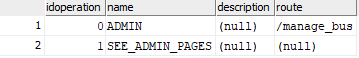
\includegraphics[scale=1]{Figs/fig6}
\end{center}

\begin{center}
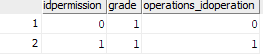
\includegraphics[scale=1]{Figs/fig7}
\end{center}

So we have two operations:
\begin{itemize}
	\item ADMIN: that allows a user to go to the page manage\_bus.
	\item SEE\_ADMIN\_PAGES: that allows a user to see the admin pages.
\end{itemize}
As you can see, the permissions are not the same: one is for a page, and the other is more general.\\

And, in the second table, we can see that both permissions are granted to the grade 1, the admin.

\subsubsection{In the website}
All the permissions are handled in the Permission middleware:\\ \emph{bus\_project/app/Http/Middleware/Permission.php}\\\

About the first one related to a page: 
\lstinputlisting[language=php, firstline=20, lastline=57, firstnumber=20]{../app/Http/Middleware/Permission.php}
\bigskip
The idea is to get the user id, then, we check his grade, and go pick all the operations is allowed to do, according to the \$operationName input. If it's allowed, it return \$next(\$request), but if it is not, it redirect the user to the home page.\\

But something is missing here... What is this variable \$operationName? Where does it come from? It comes from the routes.php file:
\lstinputlisting[language=php, firstline=55, lastline=62, firstnumber=55]{../routes/web.php}
\bigskip
Here we are! Our first route to a page!\\

As you can see, the first thing is to declare it into a Route::middleware('auth') object. Why? Because it will test if the user is logged or not. If it's not, it will redirect it to the login page without checking any other permission.\\

Then, there is the route to the manage\_bus page. And here, we can find the line 61:\\ \emph{->middleware('permission:ADMIN');}. That is your \$operationName variable from the middleware.\\

Let's talk about the second one:

This permission is to see or not the page in the navigation bar. So to see where does it come from, we need to see the file where the navigation bar is done. It is in:\\
\emph{bus\_project/resources/views/includes/aside.blade.php}
\lstinputlisting[language=php, firstline=26, lastline=57, firstnumber=26]{../resources/views/includes/aside.blade.php}
\bigskip
As it can be seen here, from line 44 to 55, there is an if clause. This clause calls a function from the middleware file, the \emph{hasOperation} function, with the parameter 'SEE\_ADMIN\_PAGES'.
\lstinputlisting[language=php, firstline=59, lastline=87, firstnumber=59]{../app/Http/Middleware/Permission.php}
\bigskip
It's done in two functions: the hasOperation function will first check if the user is logged or not. If he is not, it will return false. Else, it will call the function hasUserOperation(iduser, 'SEE\_ADMIN\_PAGES').\\

This second function will work like the one about page permission: it will check if the user has the right to perform this operation. If yes, it returns true, else it returns false.\\

We now have a working permissions handler.

\subsection{Create a bus}
Let's go back to the website and create a bus as an admin:\\

First, let's log with my admin account:
\begin{center}
	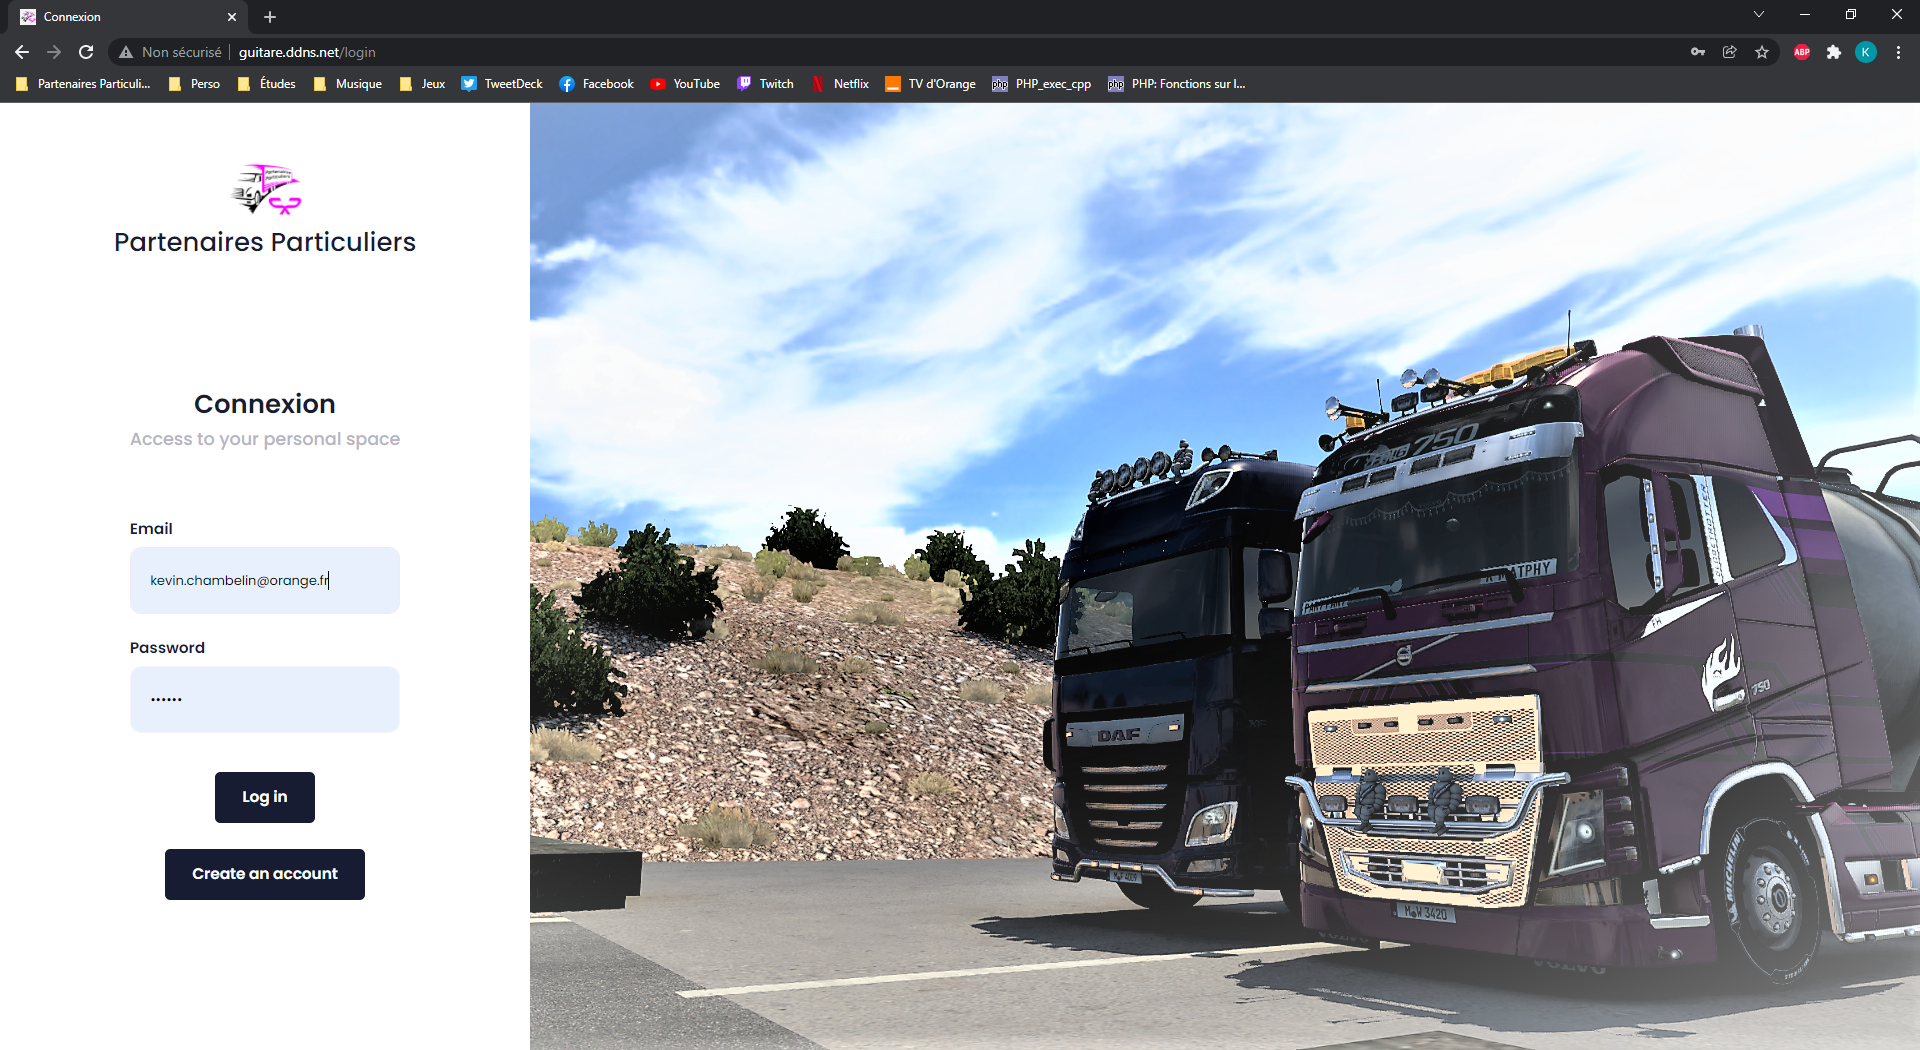
\includegraphics[scale=0.35]{Figs/fig8}
\end{center}
Now, I can see the manage bus page:
\begin{center}
	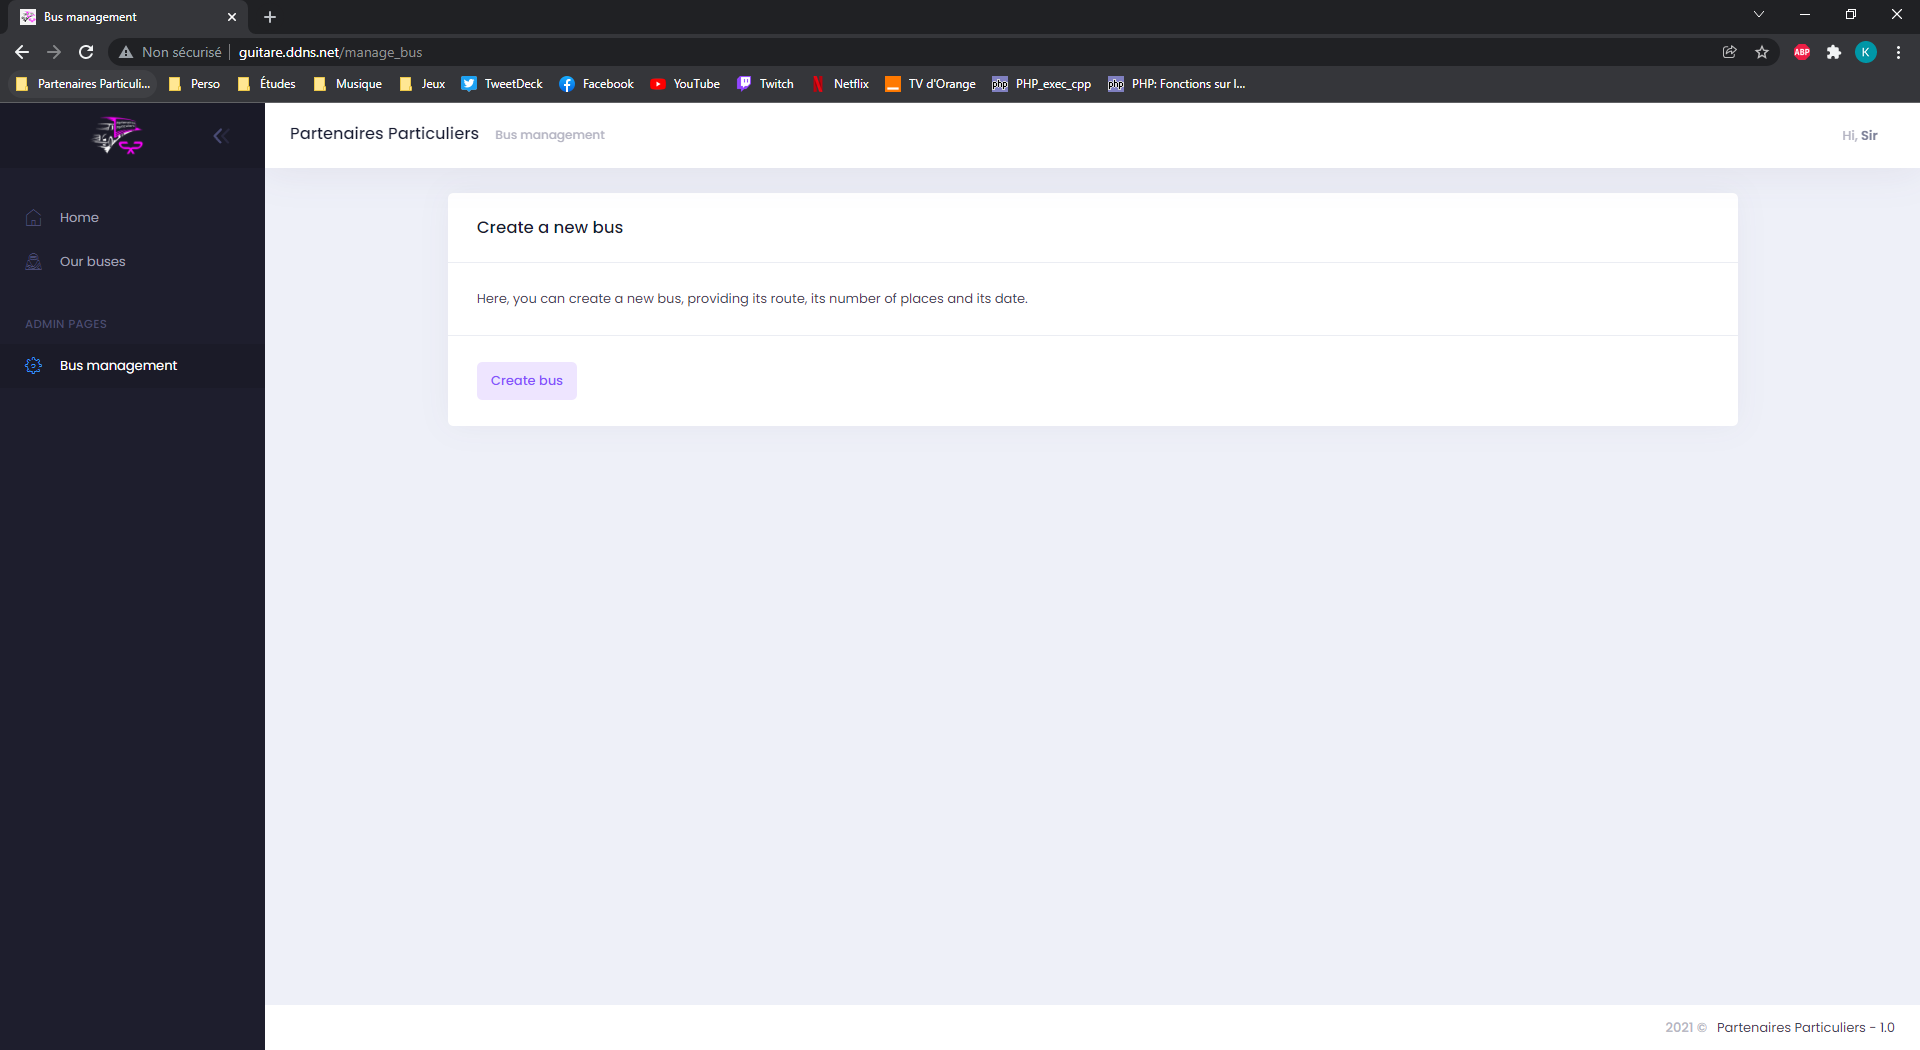
\includegraphics[scale=0.35]{Figs/fig9}
\end{center}
Let's begin the process by clicking on the Create bus button. It will open what we call a modal, that is a little window above the screen:
\begin{center}
	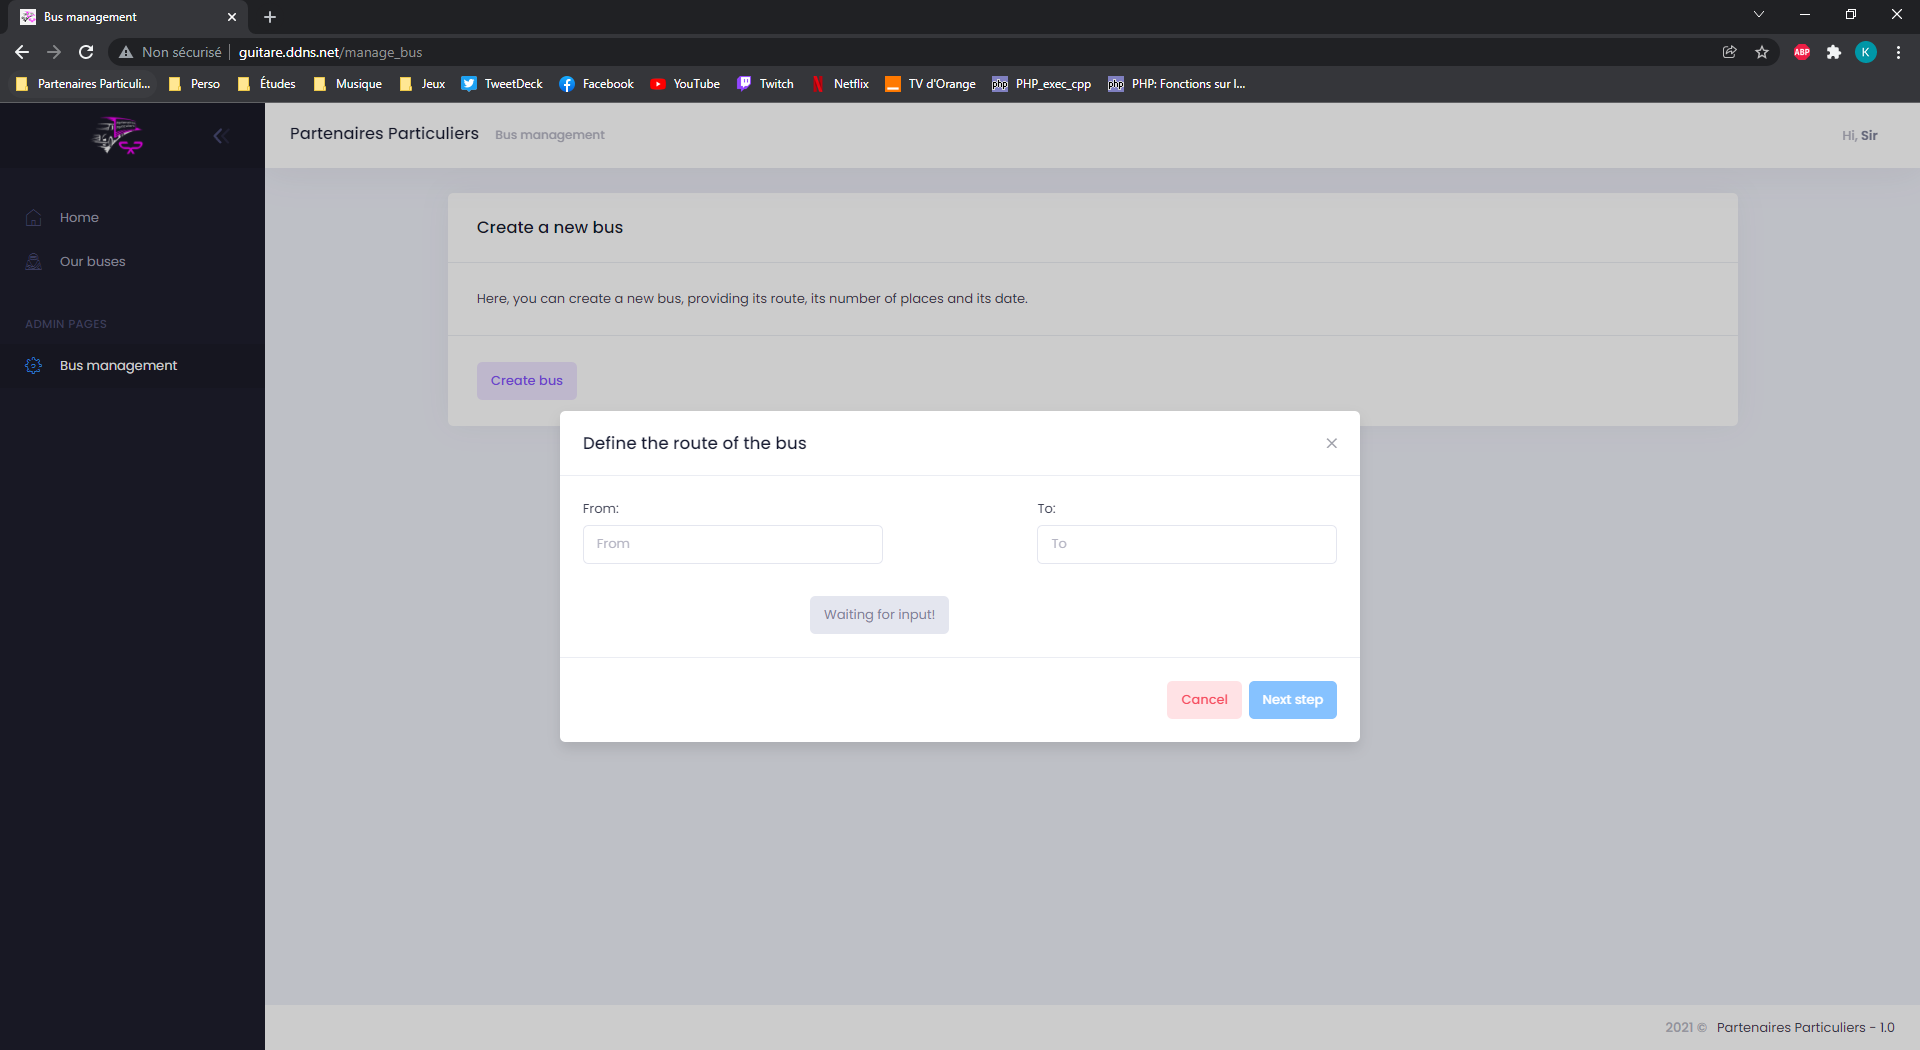
\includegraphics[scale=0.35]{Figs/fig10}
\end{center}
Here we can set the two cities for the bus. Then click on Next step to go to the next modal.

\begin{remarque}
	The next step button won't available until both inputs are correct.
\end{remarque}
\begin{center}
	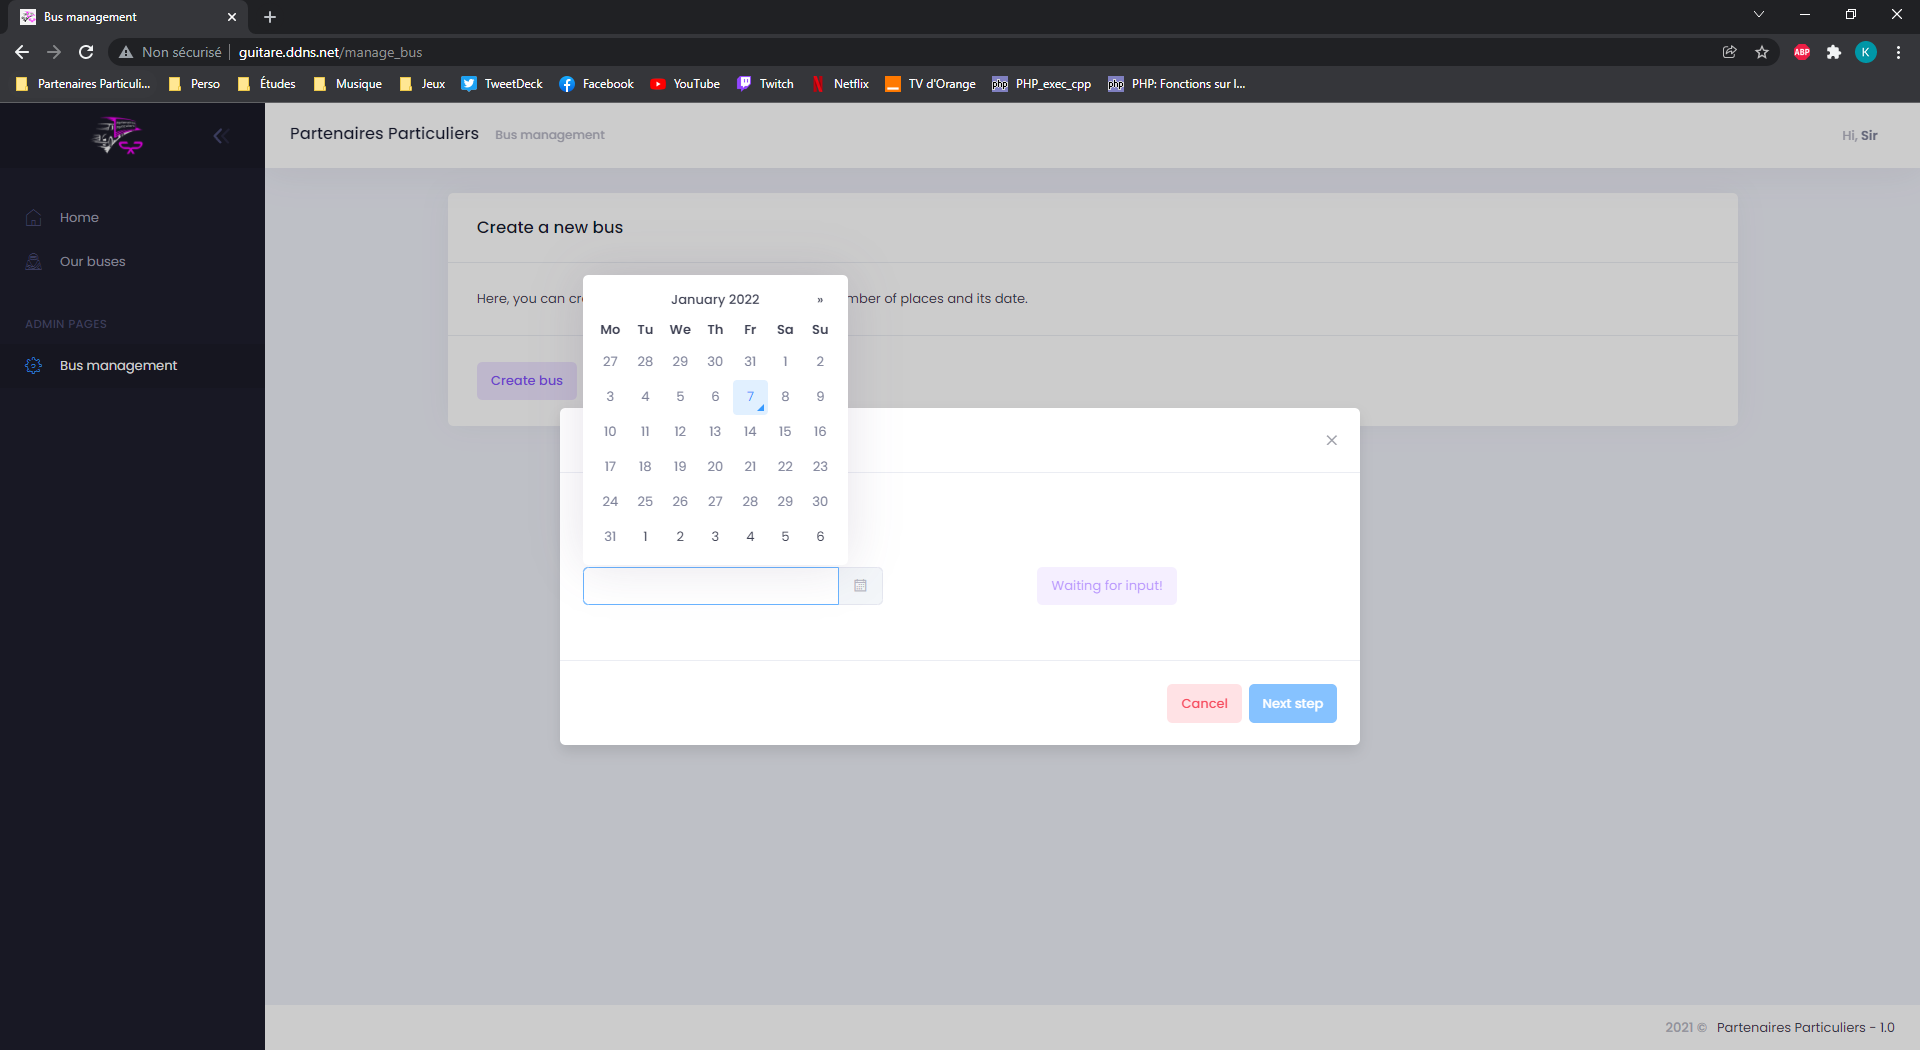
\includegraphics[scale=0.35]{Figs/fig11}
\end{center}
Then we can set the date of the bus. I put in place a protection to prevent the user to set a date before today.
\begin{center}
	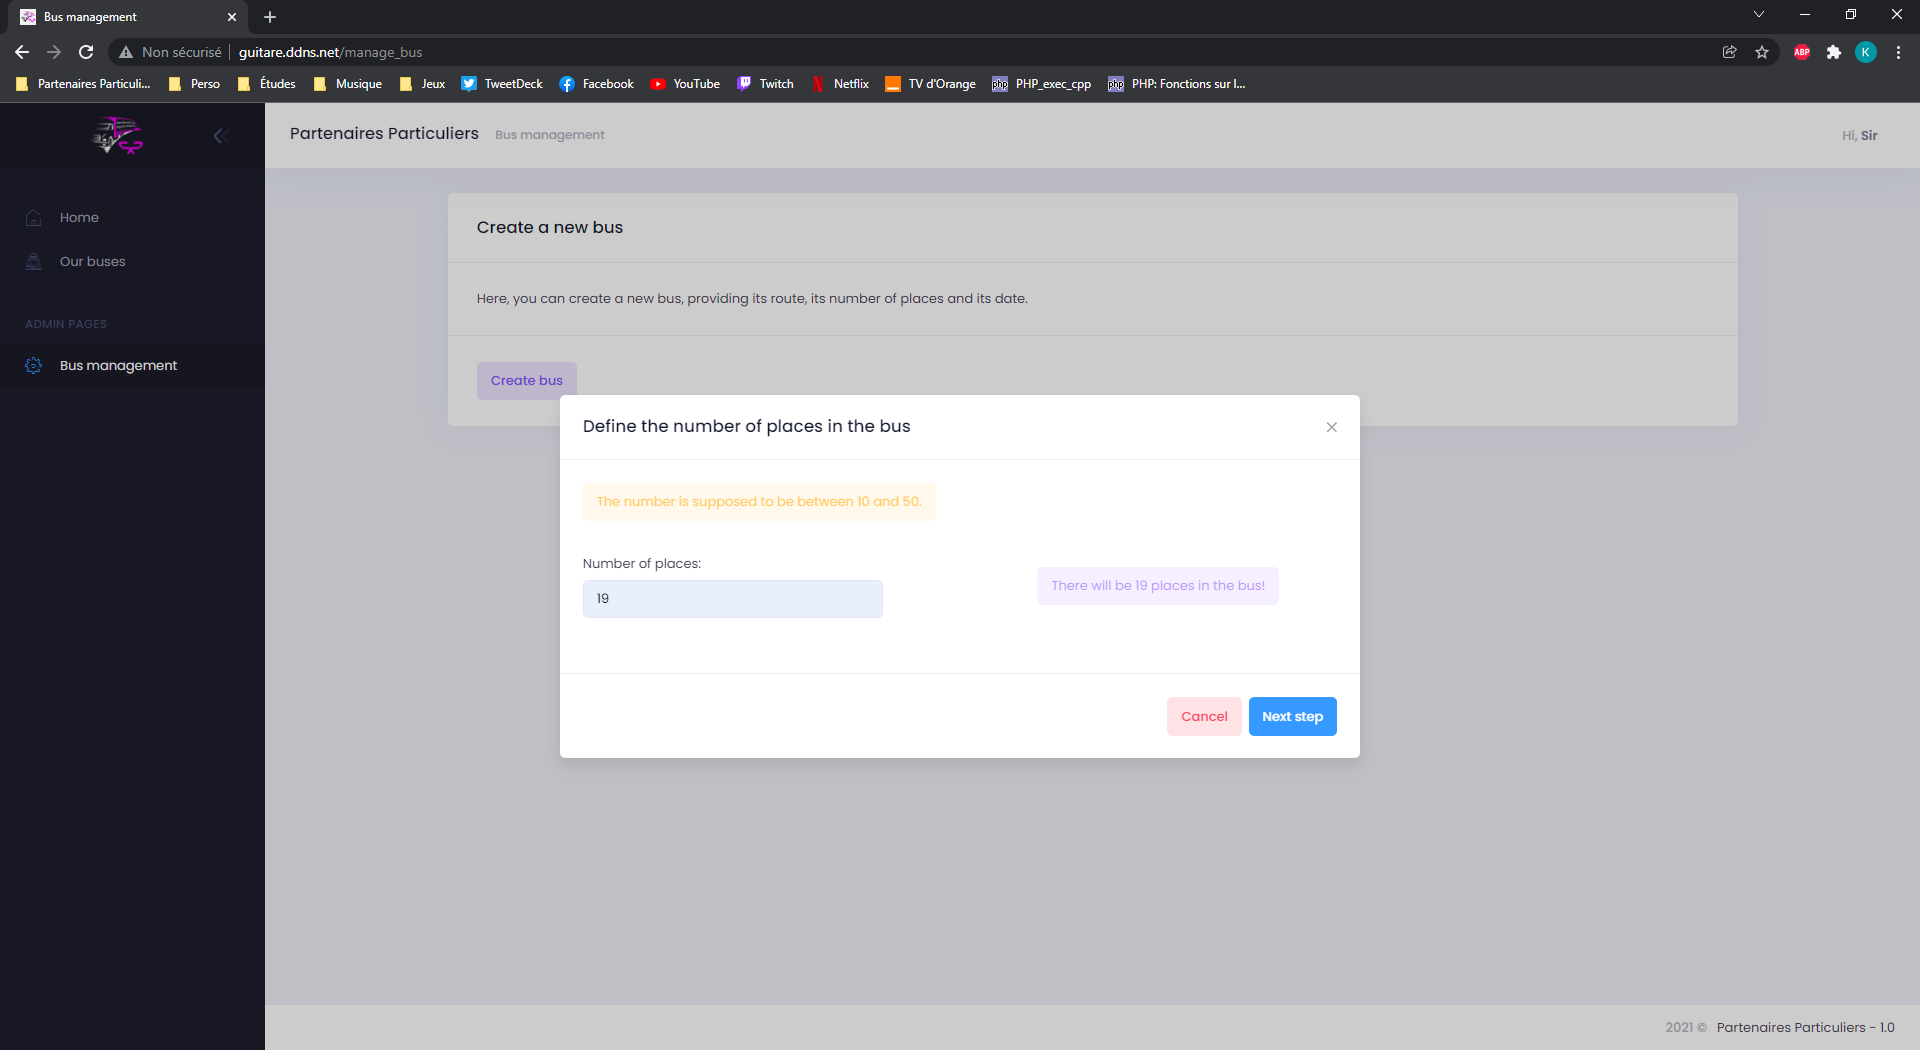
\includegraphics[scale=0.35]{Figs/fig12}
\end{center}
Here, we can set the number of places in the bus.\\

\noindent We just need to check if the data are correct. So there is a recap:
\begin{center}
	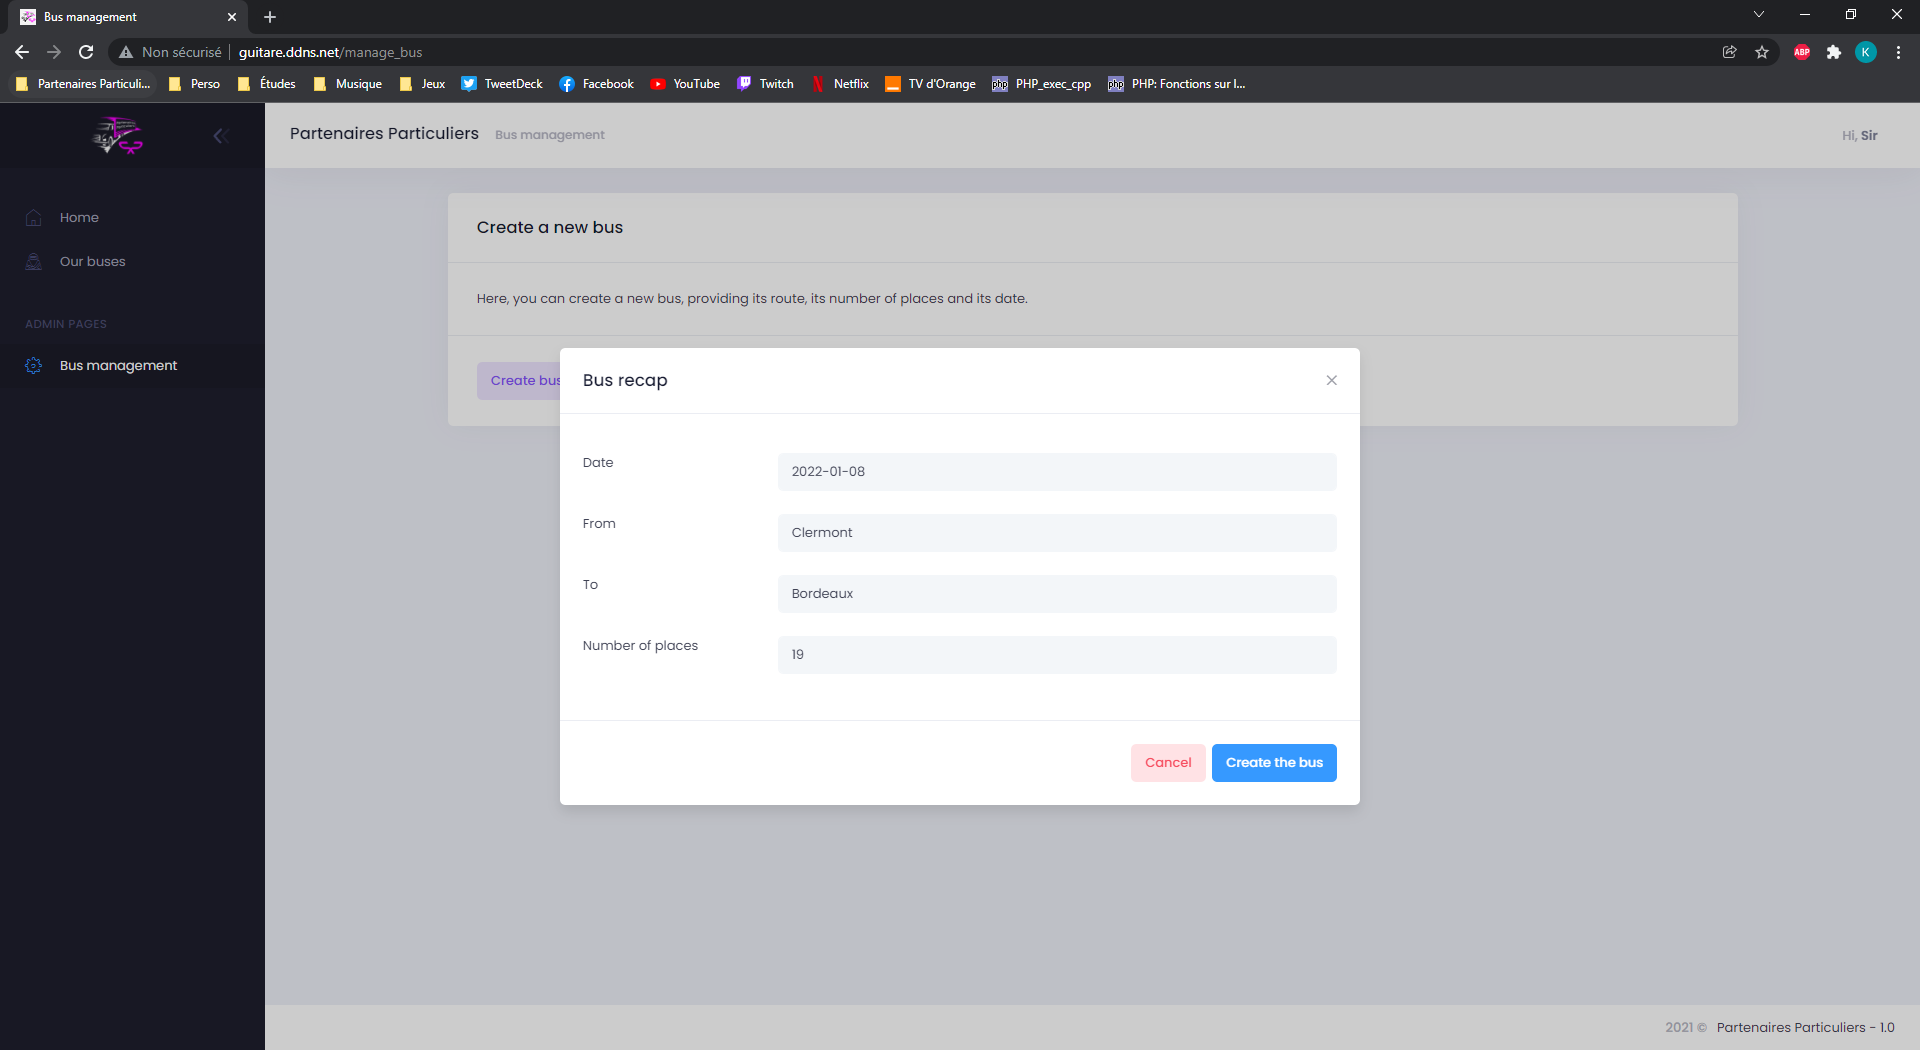
\includegraphics[scale=0.35]{Figs/fig13}
\end{center}
Now, if we click on the Create the bus button, it will trigger a JS function, as it is done for the registration. AS a reminder, JS does not have any access to the db, so we need to post the variables so that php can read and process them.\\

\noindent Here is the JS function, that you can find in:\\
\emph{bus\_project/resources/views/manage\_bus.blade.php}
\lstinputlisting[language=javascript, firstline=319, lastline=340, firstnumber=319]{../resources/views/manage_bus.blade.php}
\bigskip
As you can see, it is exactly the same process as the register one.\\

Let's see the function in the Bus controller:\\
\emph{bus\_project/app/Http/Controllers/BusController.php}
\lstinputlisting[language=php, firstline=12, lastline=31, firstnumber=12]{../app/Http/Controllers/BusController.php}
\bigskip
Once again, it's the same idea than for the registration: we save the data from AJAX in php variables, then, we get the max id of buses, and add a new record in the table.\\

Up to this point, we have achieve all the requirements in order to make our booking system. Let's do it!
\pagebreak

\subsection{The booking system -- website side}
\subsubsection{Display all the available buses}
To reserve a seat, we need to see the bus that are available, as here:
\begin{center}
	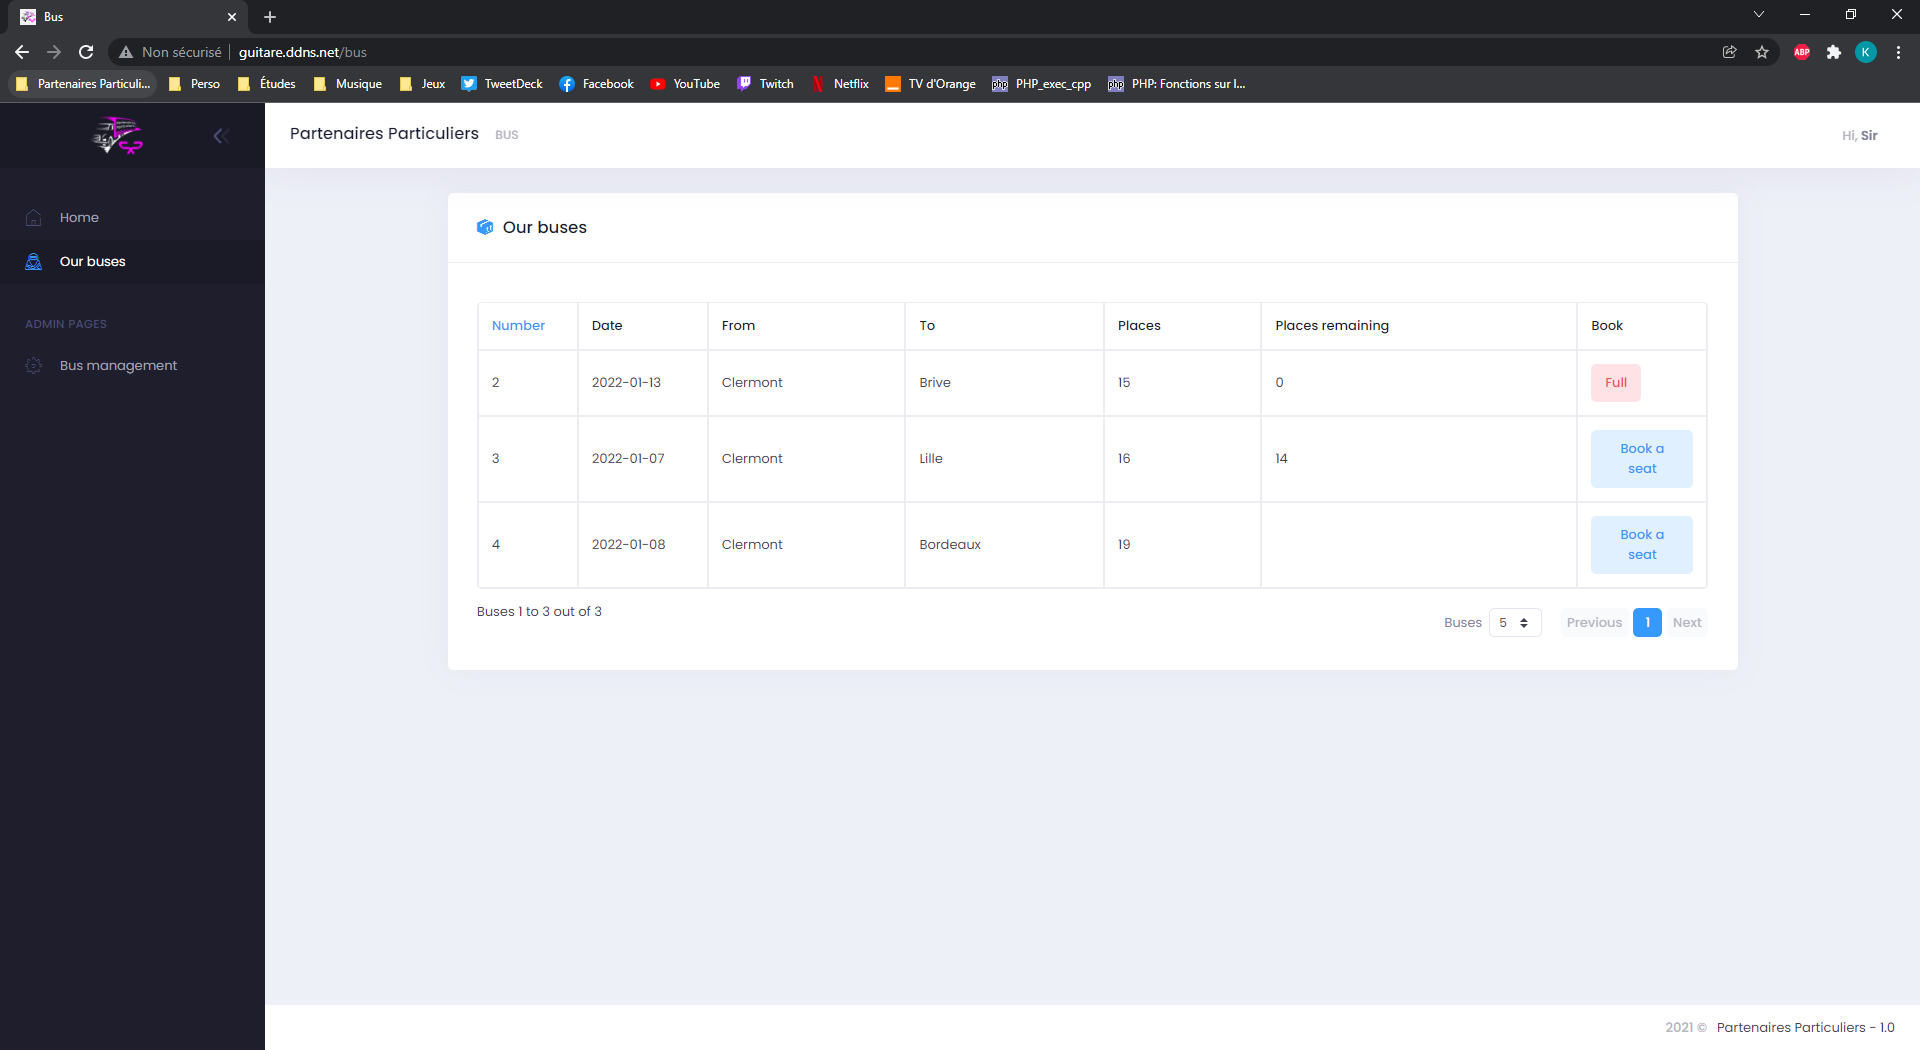
\includegraphics[scale=0.35]{Figs/fig14}
\end{center}
Here, we can all the buses that are scheduled and not yet gone. We can see how many places a bus has and how many places remain in each bus. To know that, we more "complicated" request on the db. In order to do that, I've created a SQL view. It's like a new table that is created as a result of a request. Let's see it:\\
\emph{bus\_project/DB/display\_buses.sql}
\lstinputlisting[language=sql]{../DB/display_buses.sql}
\bigskip
The request itself begins at "with purchaised..." and ends at the end of the file.\\

In the with clause we return all the places that are already reserved for each bus. The two items returned are:
\begin{itemize}
	\item bus\_idbus, the id of the bus that will be used to the incoming join.
	\item coalesce(count(idbook),0) as nb\_places, that represents the number of reserved places.
\end{itemize}
\begin{remarque}
	The coalesce keyword is used the next way:
	\emph{coalesce(smtg, 0)} will return smtg if smtg is not null, 0 otherwise.
\end{remarque}
Next, we do the select on the join of the table bus (b), and the table purchaised\_places (pp) created in the with clause, on the attribute idbus. The selected items are:
\begin{itemize}
	\item b*: all the attributes of the table bus.
	\item b.place\_number - pp.nb\_places: the number of places that remain.
\end{itemize}
With a view, Laravel will consider this as a table. So, to have the result, we just need to execute:\\
\emph{select * from display\_buses}.\\

On the website, the display of the bus is done by an AJAX request from the JS. This time, AJAX is receiving data from PHP, but it works exactly the same way as before. It uses a library called ktdatatable to display the result:\\
\emph{bus\_project/resources/views/bus.blade.php}
\lstinputlisting[language=javascript, firstline=103, lastline=197, firstnumber=103]{../resources/views/bus.blade.php}
\bigskip
The little thing that is different is for the last column, because we need either to have the book button, or to have the full tag. To do so, I made an if statement on the number of remaining places in the bus (l. 167 - 175).

\subsubsection{Booking function}
When we click on the book button, it send to the bus controller, using AJAX, the bus id and the user id. Then, all is handled by the controller:
\emph{bus\_project/app/Http/Controllers/BusController.php}
\lstinputlisting[language=php, firstline=40, lastline=80, firstnumber=40]{../app/Http/Controllers/BusController.php}
\bigskip
\hspace*{0.6cm}Here we are: the heart of the project!\\

First, we store in php variable what AJAX sent. Then begin the tricky part: calling the cpp server using sockets. The fact is that with php, the use of socket is very simple: it's handled like a file. So, in the \$fp variable, we have the socket connection. We check then if the connection worked. If it does not, return -1. Else, it wait for the Cpp server to respond. 

When the Cpp server responds, we verified the remaining places, in case somewhere else would have book while we were waiting for the cpp server. If there is still remaining places, it adds the record in the db, and returns 0 to the AJAX. Otherwise it returns -1.

Then, after the execution, the client pops a modal, with the response of the server: if the php response was 0 => success, otherwise => error, try again.
\begin{center}
	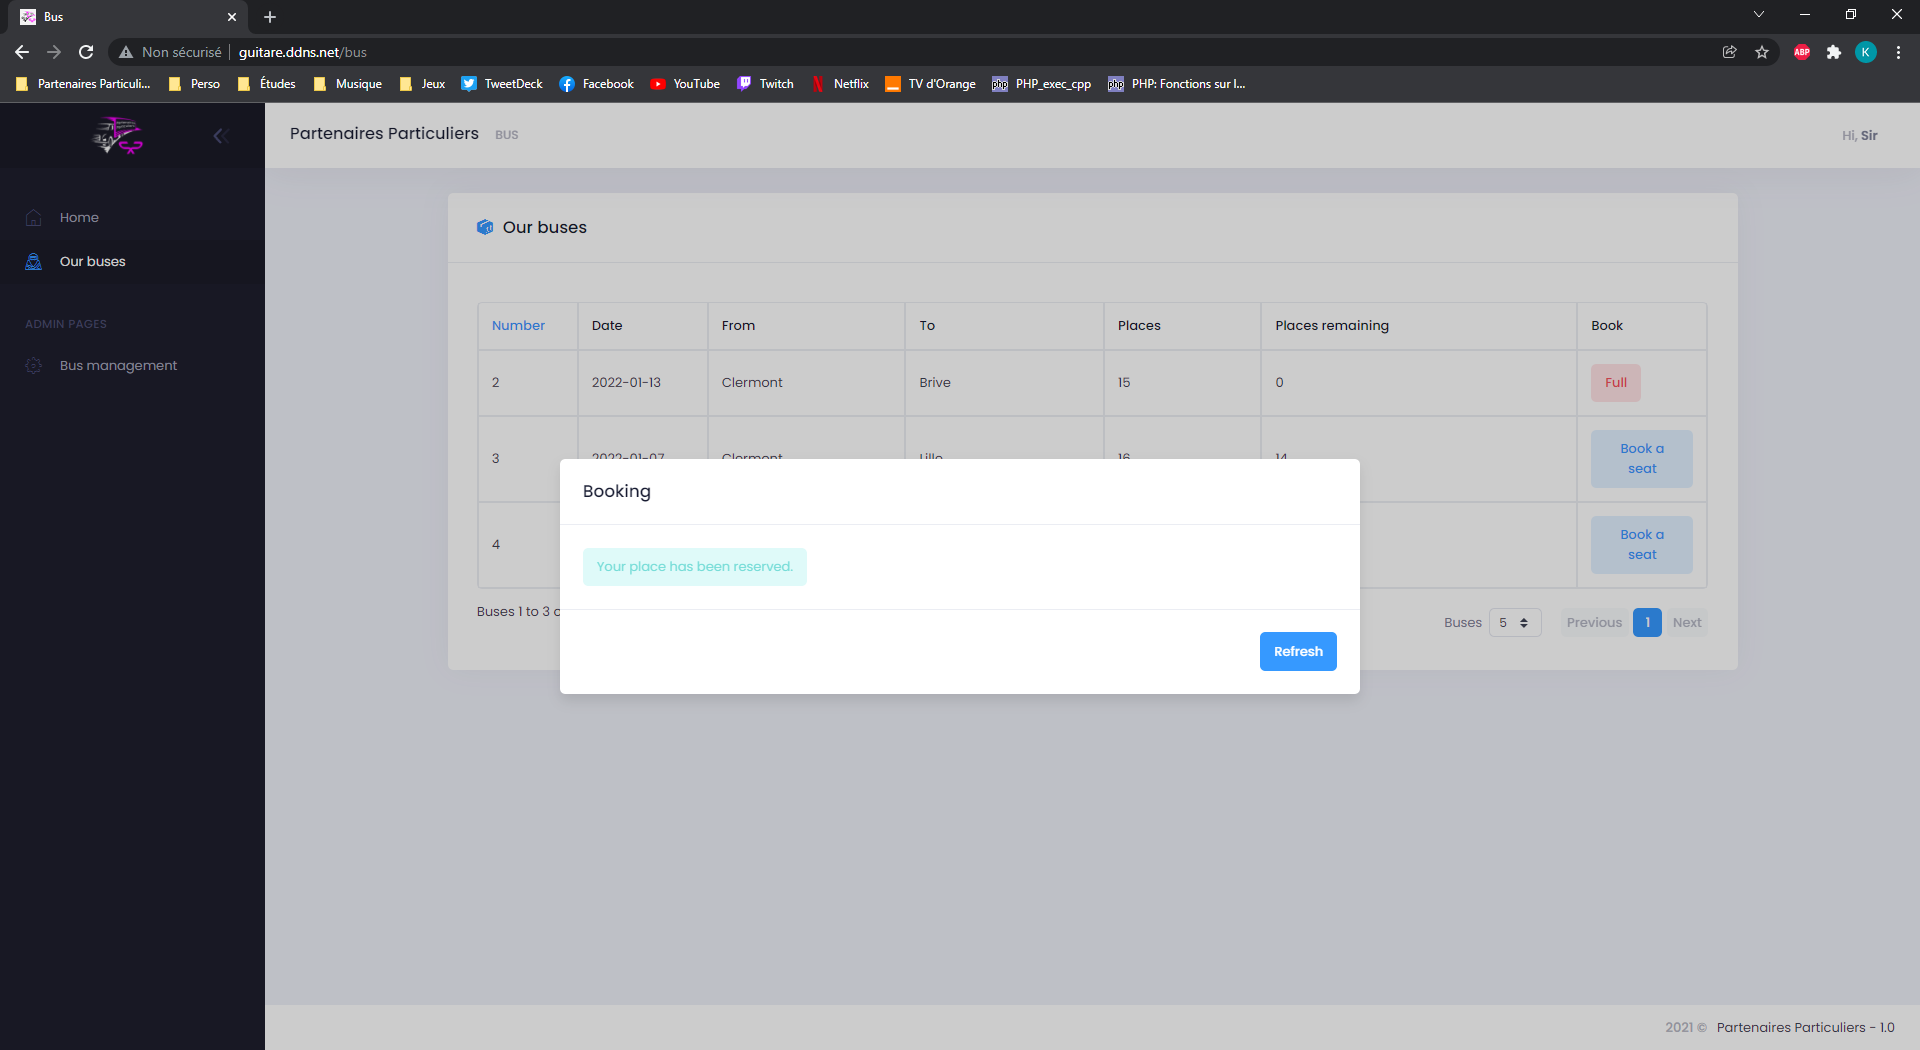
\includegraphics[scale=0.35]{Figs/fig15}
\end{center}

\section{The Cpp server}
Here is the most difficult part of the project. The mutex part, you will see, is very simple. But I had to deal with sockets multithreading, and I didn't have any idea of how this thing was working. The fact is that there is a lot of explanations and support for linux users, but no so much for windows ones... So I had to try on my own and I thing I did something not so bad.\\

To implement it, I used the winsock2 library.\\

\begin{remarque}
	In all this part, I will pick up code from the cpp file:
	\emph{Bus\_project/cpp/Server.cpp}
\end{remarque}

The first thing is to define my server class:
\lstinputlisting[language=c++, firstline=23, lastline=40, firstnumber=23]{../cpp/Server.cpp}
\bigskip
AS attributes, we have the address, the port, the state of the server and the socket. As functions, I implemented an init, a start and pause functions. I also did a function to create a thread for each connection: ThreadLauncher.\\

The constructor of the server:
\lstinputlisting[language=c++, firstline=42, lastline=45, firstnumber=42]{../cpp/Server.cpp}
\bigskip

The init() function:
\lstinputlisting[language=c++, firstline=47, lastline=76, firstnumber=47]{../cpp/Server.cpp}
\bigskip
The aim of this function is to initialize the serv by setting up the host, the port and all the necessary elements to make the server work fine.\\

One important aspect was to make it easy to debug, by adding a lot of if statements so that I know what goes wrong.

The start() function:
\lstinputlisting[language=c++, firstline=78, lastline=128, firstnumber=78]{../cpp/Server.cpp}
\bigskip
The aim of this function is to make the server listen to the port, here the 27 015. Then, as soon as it detects a new connection, it launches a new thread bound to this connection.\\

The mutex function:
\lstinputlisting[language=c++, firstline=137, lastline=149, firstnumber=137]{../cpp/Server.cpp}
\bigskip
That is the function each thread will execute. So, when a connection is detected, a thread is created and it executes it. The first thing is to lock the mutex. Then, it sends the message to php to proceed to the execution of the book. Then, it unlocks the mutex, so that another thread can lock it...

\begin{remarque}
	To be honest, I don't think that this solution will work for a huge scale project. However, there are tools available in php, or even sql, to handle real time synchronisation.
\end{remarque}
\end{document}